% ==============================================================================
% BỘ ĐỀ THAM KHẢO TUYỂN SINH 10 NĂM HỌC 2026-2027 SỞ GD&ĐT TP.HCM
% ĐỢT 21: CỤM 14 (ĐỀ 2 & ĐỀ 3 - ĐỀ SỐ 41 VÀ ĐỀ SỐ 42)
% Gồm 14 bài toán tự luận chuẩn cấu trúc tuyển sinh 10
% ==============================================================================

% ==============================================================================
% CỤM 14 - ĐỀ THAM KHẢO 2 (ĐỀ SỐ 41)
% ==============================================================================

\begin{bt}%[9D6H18-2]
% nguon: Đề tham khảo Tuyển sinh 10 năm học 2026-2027 Sở GD&ĐT TP.HCM - Cụm 14 Đề 2 (Đề số 41)
Cho hàm số $y = -\dfrac{1}{3}x^2$ có đồ thị là parabol $(P)$.
\begin{enumerate}[a)]
	\item Vẽ đồ thị $(P)$ trên hệ trục toạ độ $Oxy$.
	\item Tìm toạ độ điểm $N$ thuộc $(P)$, biết $N$ khác gốc toạ độ $O$ và có tung độ gấp ba hoành độ.
\end{enumerate}
\loigiai{
\begin{enumerate}[a)]
	\item Bảng giá trị của hàm số:
	\begin{center}
		\begin{tabular}{|c|c|c|c|c|c|}
			\hline
			$x$ & $-6$ & $-3$ & $0$ & $3$ & $6$ \\ \hline
			$y = -\dfrac{1}{3}x^2$ & $-12$ & $-3$ & $0$ & $-3$ & $-12$ \\ \hline
		\end{tabular}
	\end{center}
	Đồ thị $(P)$ là đường parabol có đỉnh tại gốc toạ độ $O(0;0)$, nhận trục tung $Oy$ làm trục đối xứng và quay bề lõm xuống dưới.
	\begin{center}
	\begin{tikzpicture}[>=stealth,scale=0.7]
		\draw[->] (-7,0) -- (7,0) node[below] {$x$};
		\draw[->] (0,-13) -- (0,2) node[left] {$y$};
		\node[above left] at (0,0) {$O$};
		\draw[dashed] (-6,0) node[above] {$-6$} -- (-6,-12) -- (0,-12) node[left] {$-12$} -- (6,-12) -- (6,0) node[above] {$6$};
		\draw[dashed] (-3,0) node[above] {$-3$} -- (-3,-3) -- (0,-3) node[left] {$-3$} -- (3,-3) -- (3,0) node[above] {$3$};
		\draw[thick,smooth,samples=100,domain=-6.2:6.2] plot(\x,{-1/3*(\x)^2});
		\fill (-6,-12) circle (1.5pt) (-3,-3) circle (1.5pt) (0,0) circle (1.5pt) (3,-3) circle (1.5pt) (6,-12) circle (1.5pt);
		\node[below right] at (3.5,-7) {$(P)\colon y = -\dfrac{1}{3}x^2$};
	\end{tikzpicture}
	\end{center}
	\item Vì điểm $N$ có tung độ gấp ba hoành độ nên ta có:
	$$y = 3x.$$
	Thay vào phương trình của $(P)$, ta được:
	$$3x = -\dfrac{1}{3}x^2 \iff \dfrac{1}{3}x^2 + 3x = 0 \iff x\left(\dfrac{1}{3}x + 3\right) = 0 \iff x = 0 \text{ hoặc } x = -9.$$
	\begin{itemize}
		\item Với $x = 0 \implies y = 0$ (loại vì $N$ khác gốc toạ độ $O$).
		\item Với $x = -9 \implies y = 3 \cdot (-9) = -27$ (nhận).
	\end{itemize}
	Vậy toạ độ điểm cần tìm là $N(-9; -27)$.
\end{enumerate}
}
\end{bt}

\begin{bt}%[9D6H20-2]
% nguon: Đề tham khảo Tuyển sinh 10 năm học 2026-2027 Sở GD&ĐT TP.HCM - Cụm 14 Đề 2 (Đề số 41)
Cho phương trình $2x^2 - 6x + 1 = 0$.
\begin{enumerate}[a)]
	\item Chứng minh phương trình luôn có hai nghiệm phân biệt $x_1, x_2$.
	\item Không giải phương trình, hãy tính giá trị của biểu thức $A = 3x_1^2 x_2 + 3x_1 x_2^2 - x_1 - x_2$.
\end{enumerate}
\loigiai{
\begin{enumerate}[a)]
	\item Phương trình $2x^2 - 6x + 1 = 0$ có các hệ số $a = 2$, $b = -6$, $c = 1$.
	Biệt thức $\Delta'$ của phương trình:
	$$\Delta' = (-3)^2 - 2 \cdot 1 = 9 - 2 = 7 > 0.$$
	Vì $\Delta' > 0$ nên phương trình luôn có hai nghiệm phân biệt $x_1, x_2$.
	\item Áp dụng định lý Viète, ta có:
	$$\begin{cases} x_1 + x_2 = -\dfrac{b}{a} = -\dfrac{-6}{2} = 3 \\ x_1 x_2 = \dfrac{c}{a} = \dfrac{1}{2}. \end{cases}$$
	Biến đổi biểu thức $A$:
	$$A = 3x_1 x_2(x_1 + x_2) - (x_1 + x_2) = (3x_1 x_2 - 1)(x_1 + x_2).$$
	Thay các giá trị của $x_1 + x_2$ và $x_1 x_2$ vào, ta được:
	$$A = \left(3 \cdot \dfrac{1}{2} - 1\right) \cdot 3 = \left(\dfrac{3}{2} - 1\right) \cdot 3 = \dfrac{1}{2} \cdot 3 = \dfrac{3}{2}.$$
	Vậy $A = \dfrac{3}{2}$.
\end{enumerate}
}
\end{bt}

\begin{bt}%[9D8H26-3]
% nguon: Đề tham khảo Tuyển sinh 10 năm học 2026-2027 Sở GD&ĐT TP.HCM - Cụm 14 Đề 2 (Đề số 41)
Biểu đồ cột kép biểu diễn số lượng học sinh tham gia giải thi đấu thể thao cấp Thành phố của một trường THCS như sau:
\begin{center}
\begin{tabular}{|l|c|c|c|c|}
	\hline
	Khối & Khối $6$ & Khối $7$ & Khối $8$ & Khối $9$ \\ \hline
	Học sinh Nam & $6$ & $9$ & $8$ & $8$ \\ \hline
	Học sinh Nữ & $8$ & $7$ & $9$ & $7$ \\ \hline
\end{tabular}
\end{center}
Nhà trường chọn ngẫu nhiên một học sinh bất kỳ tham dự ``Lễ tuyên dương thành tích thể thao''.
\begin{enumerate}[a)]
	\item Tính tổng số học sinh tham gia thi đấu thể thao của trường.
	\item Tính xác suất của biến cố $A$: ``Học sinh được chọn là học sinh nam''.
	\item Tính xác suất của biến cố $B$: ``Học sinh được chọn đang học lớp $9$''.
\end{enumerate}
\loigiai{
\begin{enumerate}[a)]
	\item Tổng số học sinh tham gia thi đấu thể thao của trường là:
	$$n(\Omega) = (6 + 8) + (9 + 7) + (8 + 9) + (8 + 7) = 14 + 16 + 17 + 15 = 62\text{ (học sinh)}.$$
	\item Tổng số học sinh nam tham gia thi đấu là:
	$$n(A) = 6 + 9 + 8 + 8 = 31\text{ (học sinh)}.$$
	Xác suất của biến cố $A$ là:
	$$P(A) = \dfrac{n(A)}{n(\Omega)} = \dfrac{31}{62} = \dfrac{1}{2}.$$
	\item Tổng số học sinh khối $9$ tham gia thi đấu là:
	$$n(B) = 8 + 7 = 15\text{ (học sinh)}.$$
	Xác suất của biến cố $B$ là:
	$$P(B) = \dfrac{n(B)}{n(\Omega)} = \dfrac{15}{62}.$$
\end{enumerate}
}
\end{bt}

\begin{bt}%[9D6V21-3]
% nguon: Đề tham khảo Tuyển sinh 10 năm học 2026-2027 Sở GD&ĐT TP.HCM - Cụm 14 Đề 2 (Đề số 41)
Người ta làm một lối đi có chiều rộng là $x$ (m) chạy dọc theo chiều dài và chiều rộng của một sân cỏ hình chữ nhật. Biết rằng sân cỏ có chiều dài $15$ m, chiều rộng $6$ m và diện tích của lối đi bằng $46\text{ m}^2$.
\begin{enumerate}[a)]
	\item Viết biểu thức tính diện tích của lối đi theo $x$.
	\item Tìm chiều rộng $x$ của lối đi.
\end{enumerate}
\loigiai{
\begin{enumerate}[a)]
	\item Kích thước của toàn bộ khu đất gồm sân cỏ và lối đi lần lượt là $x + 15$ (m) và $x + 6$ (m).
	Diện tích toàn bộ khu đất là:
	$$S_1 = (x + 15)(x + 6)\text{ (m}^2\text{)}.$$
	Diện tích của phần sân cỏ là:
	$$S_2 = 15 \cdot 6 = 90\text{ (m}^2\text{)}.$$
	Biểu thức tính diện tích của lối đi là:
	$$S = S_1 - S_2 = (x + 15)(x + 6) - 90 = x^2 + 21x + 90 - 90 = x^2 + 21x\text{ (m}^2\text{)}.$$
	\item Theo giả thiết, diện tích của lối đi bằng $46\text{ m}^2$ nên ta có phương trình:
	$$x^2 + 21x = 46 \iff x^2 + 21x - 46 = 0.$$
	Phương trình có biệt thức $\Delta = 21^2 - 4 \cdot 1 \cdot (-46) = 441 + 184 = 625 > 0 \implies \sqrt{\Delta} = 25$.
	Do đó phương trình có hai nghiệm:
	$$x_1 = \dfrac{-21 + 25}{2} = 2\text{ (nhận do } x > 0\text{)}; \quad x_2 = \dfrac{-21 - 25}{2} = -23\text{ (loại)}.$$
	Vậy chiều rộng của lối đi là $2$ m.
\end{enumerate}
}
\end{bt}

\begin{bt}%[9H0V31-3]
% nguon: Đề tham khảo Tuyển sinh 10 năm học 2026-2027 Sở GD&ĐT TP.HCM - Cụm 14 Đề 2 (Đề số 41)
Một người nông dân gánh một quang gánh gồm $2$ thúng gạo có kích thước và chứa lượng gạo như nhau. Mỗi thúng gạo có dạng nửa hình cầu đường kính $40\text{ cm}$. Để chở được nhiều gạo hơn, người nông dân đổ đầy thúng rồi vun gạo lên trên thành một hình nón có chiều cao $15\text{ cm}$.
\begin{enumerate}[a)]
	\item Tính thể tích lượng gạo chứa trong một thúng của quang gánh (làm tròn kết quả đến chữ số thập phân thứ nhất).
	\item Người nông dân dùng một lon sữa bò hình trụ có bán kính đáy $4\text{ cm}$, chiều cao $10\text{ cm}$ để đong gạo. Mỗi lần đong được lượng gạo bằng $95\%$ thể tích lon. Hỏi người nông dân cần đong ít nhất bao nhiêu lon gạo để đủ gạo cho cả hai thúng của quang gánh trên?
\end{enumerate}
\loigiai{
\begin{enumerate}[a)]
	\item Bán kính đáy của nửa hình cầu và hình nón là:
	$$R = 40 : 2 = 20\text{ (cm)}.$$
	Thể tích phần gạo chứa trong nửa hình cầu là:
	$$V_1 = \dfrac{1}{2} \cdot \dfrac{4}{3}\pi R^3 = \dfrac{2}{3}\pi \cdot 20^3 = \dfrac{16000\pi}{3}\text{ (cm}^3\text{)}.$$
	Thể tích phần gạo vun lên thành hình nón là:
	$$V_2 = \dfrac{1}{3}\pi R^2 h = \dfrac{1}{3}\pi \cdot 20^2 \cdot 15 = 2000\pi\text{ (cm}^3\text{)}.$$
	Tổng lượng gạo trong một thúng là:
	$$V = V_1 + V_2 = \dfrac{16000\pi}{3} + 2000\pi = \dfrac{22000\pi}{3} \approx 23038{,}3\text{ (cm}^3\text{)}.$$
	Vậy lượng gạo chứa trong một thúng khoảng $23038{,}3\text{ cm}^3$.
	\item Thể tích của chiếc lon sữa bò hình trụ là:
	$$V_{\text{lon}} = \pi r^2 h = \pi \cdot 4^2 \cdot 10 = 160\pi\text{ (cm}^3\text{)}.$$
	Lượng gạo thực tế đong được trong mỗi lần là:
	$$V_{\text{đong}} = 95\% \cdot 160\pi = 152\pi\text{ (cm}^3\text{)}.$$
	Tổng lượng gạo của cả hai thúng trong quang gánh là:
	$$V_{\text{tổng}} = 2V = 2 \cdot \dfrac{22000\pi}{3} = \dfrac{44000\pi}{3}\text{ (cm}^3\text{)}.$$
	Số lon gạo cần đong là:
	$$N = \dfrac{V_{\text{tổng}}}{V_{\text{đong}}} = \dfrac{\dfrac{44000\pi}{3}}{152\pi} = \dfrac{44000}{456} \approx 96{,}49\text{ (lon)}.$$
	Vì số lon đong phải là số nguyên nên người nông dân cần đong ít nhất $97$ lon gạo.
\end{enumerate}
}
\end{bt}

\begin{bt}%[9D1H3-4]
% nguon: Đề tham khảo Tuyển sinh 10 năm học 2026-2027 Sở GD&ĐT TP.HCM - Cụm 14 Đề 2 (Đề số 41)
Lớp 9A có $27$ học sinh nam và $18$ học sinh nữ. Nhân dịp sinh nhật của bạn An (là một học sinh nam trong lớp), các bạn trong lớp tự làm quà tặng bạn An. Mỗi bạn nam của lớp làm $3$ tấm thiệp, mỗi bạn nữ xếp $2$ hoặc $5$ con hạc giấy. Biết tổng số tấm thiệp và tổng số con hạc giấy bằng nhau (bạn An không tự làm quà tặng mình). Hỏi có bao nhiêu bạn nữ xếp $2$ con hạc và bao nhiêu bạn nữ xếp $5$ con hạc?
\loigiai{
Gọi $x$ là số bạn nữ xếp $2$ con hạc và $y$ là số bạn nữ xếp $5$ con hạc ($x, y \in \mathbb{N}, x, y \le 18$).
Vì tổng số bạn nữ trong lớp là $18$ bạn nên ta có phương trình:
$$x + y = 18. \quad (1)$$
Vì bạn An là học sinh nam nên số bạn nam tham gia làm thiệp tặng quà là:
$$27 - 1 = 26\text{ (bạn)}.$$
Tổng số tấm thiệp các bạn nam làm là:
$$26 \cdot 3 = 78\text{ (tấm)}.$$
Tổng số con hạc các bạn nữ xếp là:
$$2x + 5y\text{ (con)}.$$
Vì tổng số con hạc bằng tổng số tấm thiệp nên ta có phương trình:
$$2x + 5y = 78. \quad (2)$$
Từ $(1)$ và $(2)$ ta có hệ phương trình:
$$\begin{cases} x + y = 18 \\ 2x + 5y = 78 \end{cases} \iff \begin{cases} 2x + 2y = 36 \\ 2x + 5y = 78 \end{cases} \iff \begin{cases} 3y = 42 \\ x + y = 18 \end{cases} \iff \begin{cases} y = 14 \\ x = 4 \end{cases}\text{ (thoả mãn)}.$$
Vậy có $4$ bạn nữ xếp $2$ con hạc và $14$ bạn nữ xếp $5$ con hạc.
}
\end{bt}

\begin{bt}%[9H9C29-3]
% nguon: Đề tham khảo Tuyển sinh 10 năm học 2026-2027 Sở GD&ĐT TP.HCM - Cụm 14 Đề 2 (Đề số 41)
Cho đường tròn $(O; R)$ và đường thẳng $d$ không cắt $(O)$. Dựng đường thẳng $OH$ vuông góc với $d$ tại $H$. Trên đường thẳng $d$ lấy điểm $K$ ($K$ khác $H$), qua $K$ vẽ hai tiếp tuyến $KA, KB$ của $(O)$ ($A, B$ là các tiếp điểm) sao cho $A$ và $H$ nằm về hai phía của đường thẳng $OK$.
\begin{enumerate}[a)]
	\item Chứng minh tứ giác $KAOH$ nội tiếp đường tròn.
	\item Đường thẳng $AB$ cắt đường thẳng $OH$ tại $I$. Chứng minh $IA \cdot IB = IH \cdot IO$.
	\item Khi $OK = 2R$ và $OH = R\sqrt{3}$, hãy tính diện tích tam giác $KAB$ theo $R$.
\end{enumerate}
\loigiai{
\begin{center}
\begin{tikzpicture}[>=stealth,scale=1.1]
	\def\R{2.2}
	\coordinate (O) at (0,0);
	\draw[thick] (O) circle (\R);
	% K ở (3.5, 0.5)
	\coordinate (K) at (3.5,0.5);
	\coordinate (H) at (0,-2.6);
	\draw (O) -- (0,-3.2);
	\draw (-2,-2.6) -- (4.5,-2.6) node[right] {$d$};
	\draw (O) -- (K);
	% Tiếp tuyến KA, KB
	\coordinate (A) at ({2.2*cos(59.6)},{2.2*sin(59.6)});
	\coordinate (B) at ({2.2*cos(-43.4)},{2.2*sin(-43.4)});
	\draw (K) -- (A) -- (O) -- (B) -- (K);
	\draw (A) -- (B);
	\draw (K) -- (H);
	\coordinate (M) at (intersection of O--K and A--B);
	% Giao điểm I của AB và đường thẳng OH (trục tung)
	\coordinate (I) at (intersection of A--B and O--H);
	\draw (B) -- (I);
	\draw (O) -- (I);
	% Ký hiệu
	\fill (O) circle (1.5pt) node[above left] {$O$}
		  (K) circle (1.5pt) node[right] {$K$}
		  (H) circle (1.5pt) node[below left] {$H$}
		  (A) circle (1.5pt) node[above] {$A$}
		  (B) circle (1.5pt) node[below right] {$B$}
		  (M) circle (1.5pt) node[above right] {$M$}
		  (I) circle (1.5pt) node[left] {$I$};
\end{tikzpicture}
\end{center}
\begin{enumerate}[a)]
	\item Vì $KA$ là tiếp tuyến của $(O)$ tại $A$ nên $KA \perp OA \implies \widehat{KAO} = 90^\circ$.
	Tam giác $KAO$ vuông tại $A$ nên nội tiếp đường tròn đường kính $KO$.
	Lại có $OH \perp d$ tại $H$ nên $\widehat{KHO} = 90^\circ$.
	Tam giác $KHO$ vuông tại $H$ nên nội tiếp đường tròn đường kính $KO$.
	Suy ra bốn điểm $K, A, O, H$ cùng thuộc đường tròn đường kính $KO$, do đó tứ giác $KAOH$ nội tiếp.
	\item Vì $KB$ là tiếp tuyến của $(O)$ tại $B$ nên $KB \perp OB \implies \widehat{KBO} = 90^\circ$.
	Tam giác $KBO$ vuông tại $B$ nên nội tiếp đường tròn đường kính $KO$.
	Kết hợp với câu a, ta có $5$ điểm $K, A, O, B, H$ cùng thuộc đường tròn đường kính $KO$.
	Suy ra tứ giác $AOHB$ nội tiếp.
	Xét $\triangle IAH$ và $\triangle IOB$ có:
	\begin{itemize}
		\item $\widehat{AIH} = \widehat{OIB}$ (hai góc đối đỉnh);
		\item $\widehat{IAH} = \widehat{IOB}$ (hai góc nội tiếp cùng chắn cung $BH$).
	\end{itemize}
	Do đó $\triangle IAH \sim \triangle IOB$ (g-g).
	Suy ra $\dfrac{IA}{IO} = \dfrac{IH}{IB} \implies IA \cdot IB = IH \cdot IO$.
	\item Gọi $M$ là giao điểm của $OK$ và $AB$.
	Theo tính chất hai tiếp tuyến cắt nhau, ta có $KA = KB$ và $OA = OB = R$, nên $OK$ là đường trung trực của đoạn thẳng $AB$, do đó $OK \perp AB$ tại $M$.
	Xét tam giác vuông $OAK$ tại $A$, có đường cao $AM$:
	$$AK = \sqrt{OK^2 - OA^2} = \sqrt{(2R)^2 - R^2} = R\sqrt{3}.$$
	Áp dụng hệ thức lượng trong tam giác vuông $OAK$, ta có:
	$$OM = \dfrac{OA^2}{OK} = \dfrac{R^2}{2R} = \dfrac{R}{2}.$$
	$$AM = \dfrac{OA \cdot AK}{OK} = \dfrac{R \cdot R\sqrt{3}}{2R} = \dfrac{R\sqrt{3}}{2}.$$
	Vì $OK$ là trung trực của $AB$ nên $M$ là trung điểm của $AB$, suy ra:
	$$AB = 2AM = 2 \cdot \dfrac{R\sqrt{3}}{2} = R\sqrt{3}.$$
	Độ dài đoạn thẳng $KM$ là:
	$$KM = OK - OM = 2R - \dfrac{R}{2} = \dfrac{3R}{2}.$$
	Diện tích tam giác $KAB$ là:
	$$S_{\triangle KAB} = \dfrac{1}{2} KM \cdot AB = \dfrac{1}{2} \cdot \dfrac{3R}{2} \cdot R\sqrt{3} = \dfrac{3R^2\sqrt{3}}{4}.$$
	Vậy diện tích tam giác $KAB$ là $\dfrac{3R^2\sqrt{3}}{4}$.
\end{enumerate}
}
\end{bt}

% ==============================================================================
% CỤM 14 - ĐỀ THAM KHẢO 3 (ĐỀ SỐ 42)
% ==============================================================================

\begin{bt}%[9D6H18-2]
% nguon: Đề tham khảo Tuyển sinh 10 năm học 2026-2027 Sở GD&ĐT TP.HCM - Cụm 14 Đề 3 (Đề số 42)
Cho hàm số $y = x^2$ có đồ thị là parabol $(P)$.
\begin{enumerate}[a)]
	\item Vẽ đồ thị $(P)$ trên hệ trục toạ độ $Oxy$.
	\item Tìm toạ độ các điểm thuộc đồ thị $(P)$ có tung độ bằng $12$.
\end{enumerate}
\loigiai{
\begin{enumerate}[a)]
	\item Bảng giá trị của hàm số:
	\begin{center}
		\begin{tabular}{|c|c|c|c|c|c|}
			\hline
			$x$ & $-2$ & $-1$ & $0$ & $1$ & $2$ \\ \hline
			$y = x^2$ & $4$ & $1$ & $0$ & $1$ & $4$ \\ \hline
		\end{tabular}
	\end{center}
	Đồ thị $(P)$ là đường parabol có đỉnh tại gốc toạ độ $O(0;0)$, nhận trục tung $Oy$ làm trục đối xứng và quay bề lõm lên trên.
	\begin{center}
	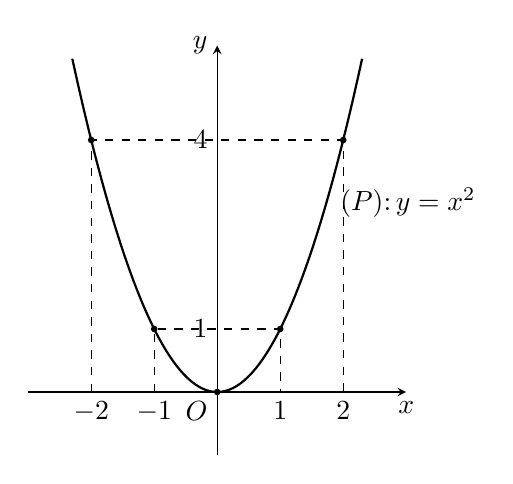
\begin{tikzpicture}[>=stealth,scale=0.8]
		\draw[->] (-3,0) -- (3,0) node[below] {$x$};
		\draw[->] (0,-1) -- (0,5.5) node[left] {$y$};
		\node[below left] at (0,0) {$O$};
		\draw[dashed] (-2,0) node[below] {$-2$} -- (-2,4) -- (0,4) node[left] {$4$} -- (2,4) -- (2,0) node[below] {$2$};
		\draw[dashed] (-1,0) node[below] {$-1$} -- (-1,1) -- (0,1) node[left] {$1$} -- (1,1) -- (1,0) node[below] {$1$};
		\draw[thick,smooth,samples=100,domain=-2.3:2.3] plot(\x,{(\x)^2});
		\fill (-2,4) circle (1.5pt) (-1,1) circle (1.5pt) (0,0) circle (1.5pt) (1,1) circle (1.5pt) (2,4) circle (1.5pt);
		\node[right] at (1.8,3) {$(P)\colon y = x^2$};
	\end{tikzpicture}
	\end{center}
	\item Vì điểm cần tìm thuộc $(P)$ và có tung độ bằng $12$ nên thay $y = 12$ vào phương trình hàm số ta có:
	$$x^2 = 12 \iff x = 2\sqrt{3} \text{ hoặc } x = -2\sqrt{3}.$$
	Vậy toạ độ các điểm cần tìm là $(2\sqrt{3}; 12)$ và $(-2\sqrt{3}; 12)$.
\end{enumerate}
}
\end{bt}

\begin{bt}%[9D6H20-2]
% nguon: Đề tham khảo Tuyển sinh 10 năm học 2026-2027 Sở GD&ĐT TP.HCM - Cụm 14 Đề 3 (Đề số 42)
Cho phương trình $x^2 - 3x - 10 = 0$.
\begin{enumerate}[a)]
	\item Chứng tỏ phương trình luôn có hai nghiệm phân biệt $x_1, x_2$.
	\item Không giải phương trình, hãy tính giá trị của biểu thức $Q = \dfrac{x_1 + 1}{x_2} + \dfrac{x_2 + 1}{x_1}$.
\end{enumerate}
\loigiai{
\begin{enumerate}[a)]
	\item Phương trình $x^2 - 3x - 10 = 0$ có các hệ số $a = 1$, $b = -3$, $c = -10$.
	Biệt thức $\Delta$ của phương trình là:
	$$\Delta = b^2 - 4ac = (-3)^2 - 4 \cdot 1 \cdot (-10) = 9 + 40 = 49 > 0.$$
	Vì $\Delta > 0$ nên phương trình luôn có hai nghiệm phân biệt $x_1, x_2$.
	\item Theo định lý Viète, ta có:
	$$\begin{cases} x_1 + x_2 = -\dfrac{b}{a} = 3 \\ x_1 x_2 = \dfrac{c}{a} = -10. \end{cases}$$
	Ta có:
	$$x_1^2 + x_2^2 = (x_1 + x_2)^2 - 2x_1 x_2 = 3^2 - 2(-10) = 9 + 20 = 29.$$
	Biến đổi biểu thức $Q$:
	\begin{align*}
		Q &= \dfrac{x_1(x_1 + 1) + x_2(x_2 + 1)}{x_1 x_2} \\
		&= \dfrac{x_1^2 + x_1 + x_2^2 + x_2}{x_1 x_2} \\
		&= \dfrac{(x_1^2 + x_2^2) + (x_1 + x_2)}{x_1 x_2}.
	\end{align*}
	Thay các giá trị tương ứng vào, ta được:
	$$Q = \dfrac{29 + 3}{-10} = \dfrac{32}{-10} = -\dfrac{16}{5}.$$
	Vậy $Q = -\dfrac{16}{5}$.
\end{enumerate}
}
\end{bt}

\begin{bt}%[9D8H26-3]
% nguon: Đề tham khảo Tuyển sinh 10 năm học 2026-2027 Sở GD&ĐT TP.HCM - Cụm 14 Đề 3 (Đề số 42)
\begin{enumerate}[a)]
	\item Bạn Minh hỏi $40$ bạn học sinh bất kỳ về môn học mà bạn đó yêu thích nhất. Kết quả thống kê thu được: Toán có $11$ bạn, Ngữ văn có $8$ bạn, Lịch sử có $9$ bạn, Thể dục có $12$ bạn. Hãy chỉ ra tần số và tính tần số tương đối của môn Lịch sử.
	\item Trong một hộp có $20$ chiếc thẻ cùng loại được đánh số từ $1$ đến $20$. Bạn Hà rút ngẫu nhiên một thẻ trong hộp. Hãy tính xác suất của biến cố $A$: ``Số ghi trên thẻ là số lớn hơn $15$''.
\end{enumerate}
\loigiai{
\begin{enumerate}[a)]
	\item Tần số của môn Lịch sử là $9$.
	Tần số tương đối của môn Lịch sử là:
	$$f = \dfrac{9}{40} \cdot 100\% = 22{,}5\%.$$
	\item Số phần tử của không gian mẫu khi rút ngẫu nhiên $1$ thẻ từ $20$ thẻ là:
	$$n(\Omega) = 20.$$
	Biến cố $A$: ``Số ghi trên thẻ lớn hơn $15$''.
	Các kết quả thuận lợi cho biến cố $A$ là các số $16; 17; 18; 19; 20$.
	Số kết quả thuận lợi cho biến cố $A$ là $n(A) = 5$.
	Xác suất của biến cố $A$ là:
	$$P(A) = \dfrac{n(A)}{n(\Omega)} = \dfrac{5}{20} = \dfrac{1}{4}.$$
\end{enumerate}
}
\end{bt}

\begin{bt}%[9D6V21-3]
% nguon: Đề tham khảo Tuyển sinh 10 năm học 2026-2027 Sở GD&ĐT TP.HCM - Cụm 14 Đề 3 (Đề số 42)
Một cái sân hình chữ nhật có chiều dài là $1{,}57x + 10$ (m). Ở góc sân, người ta làm một bồn hoa hình tròn có bán kính $x$ (m) ($x > 0$). Biết bồn hoa tiếp xúc với hai cạnh góc vuông của sân và cách cạnh chiều dài còn lại của sân một khoảng bằng $2$ m.
\begin{enumerate}[a)]
	\item Viết biểu thức biểu thị diện tích phần đất còn lại sau khi đã xây bồn hoa theo $x$ và $\pi$.
	\item Tính bán kính $x$ của bồn hoa, biết diện tích phần đất còn lại là $54{,}71\text{ m}^2$ (lấy $\pi \approx 3{,}14$).
\end{enumerate}
\loigiai{
\begin{enumerate}[a)]
	\item Vì bồn hoa hình tròn bán kính $x$ tiếp xúc với một cạnh chiều dài và cách cạnh chiều dài đối diện một khoảng $2$ m, nên chiều rộng của sân hình chữ nhật là:
	$$x + x + 2 = 2x + 2\text{ (m)}.$$
	Diện tích của toàn bộ sân hình chữ nhật là:
	$$S_{\text{sân}} = (1{,}57x + 10)(2x + 2)\text{ (m}^2\text{)}.$$
	Diện tích của bồn hoa hình tròn là:
	$$S_{\text{hoa}} = \pi x^2\text{ (m}^2\text{)}.$$
	Diện tích phần đất còn lại của sân là:
	$$S = S_{\text{sân}} - S_{\text{hoa}} = (1{,}57x + 10)(2x + 2) - \pi x^2\text{ (m}^2\text{)}.$$
	\item Thay $\pi \approx 3{,}14$ và $S = 54{,}71$ vào biểu thức, ta có phương trình:
	$$(1{,}57x + 10)(2x + 2) - 3{,}14x^2 = 54{,}71$$
	$$\iff 3{,}14x^2 + 3{,}14x + 20x + 20 - 3{,}14x^2 = 54{,}71$$
	$$\iff 23{,}14x + 20 = 54{,}71$$
	$$\iff 23{,}14x = 34{,}71$$
	$$\iff x = \dfrac{34{,}71}{23{,}14} = 1{,}5\text{ (m)}.$$
	Vậy bán kính của bồn hoa hình tròn là $1{,}5$ m.
\end{enumerate}
}
\end{bt}

\begin{bt}%[9H0V31-3]
% nguon: Đề tham khảo Tuyển sinh 10 năm học 2026-2027 Sở GD&ĐT TP.HCM - Cụm 14 Đề 3 (Đề số 42)
Người ta xếp hai quả bóng hình cầu có cùng bán kính $R$ vào một chiếc hộp hình trụ sao cho các quả bóng đều tiếp xúc với hai đáy, đồng thời hai quả bóng tiếp xúc với nhau và mỗi quả bóng đều tiếp xúc với đường sinh của hình trụ. Biết thể tích của chiếc hộp hình trụ là $120\text{ cm}^3$. Tính thể tích của mỗi quả bóng.
\loigiai{
Vì hai quả bóng tiếp xúc với nhau và mỗi quả bóng tiếp xúc với một đáy của hình trụ nên chiều cao của hình trụ là:
$$h = 2R + 2R = 4R \text{ (hoặc nếu hai quả bóng đặt cạnh nhau theo phương ngang thì } h = 2R\text{)}.$$
Theo giả thiết hình vẽ, hai quả bóng đặt cạnh nhau trên đáy hình trụ và cùng tiếp xúc với hai mặt đáy:
Chiều cao của hình trụ bằng đường kính của mỗi quả bóng:
$$h = 2R.$$
Vì hai quả bóng tiếp xúc nhau và tiếp xúc với thành trụ nên đường kính đáy của hình trụ bằng tổng đường kính hai quả bóng:
$$2R_{\text{trụ}} = 2R + 2R = 4R \implies R_{\text{trụ}} = 2R.$$
Thể tích của chiếc hộp hình trụ là:
$$V_{\text{trụ}} = \pi R_{\text{trụ}}^2 h = \pi (2R)^2 \cdot 2R = 8\pi R^3.$$
Theo đề bài:
$$8\pi R^3 = 120 \implies \pi R^3 = \dfrac{120}{8} = 15\text{ (cm}^3\text{)}.$$
Thể tích của mỗi quả bóng hình cầu là:
$$V_{\text{cầu}} = \dfrac{4}{3}\pi R^3 = \dfrac{4}{3} \cdot 15 = 20\text{ (cm}^3\text{)}.$$
Vậy thể tích của mỗi quả bóng là $20\text{ cm}^3$.
}
\end{bt}

\begin{bt}%[9D1H3-4]
% nguon: Đề tham khảo Tuyển sinh 10 năm học 2026-2027 Sở GD&ĐT TP.HCM - Cụm 14 Đề 3 (Đề số 42)
Bác An vay tại một ngân hàng $100$ triệu đồng để sản xuất trong thời hạn một năm. Hết năm thứ nhất, do làm ăn gặp khó khăn nên bác được ngân hàng gia hạn thêm một năm nữa với lãi suất không đổi; số tiền lãi của năm đầu được gộp vào vốn để tính lãi năm sau. Hết hai năm, bác An phải trả cho ngân hàng tất cả $118\,810\,000$ đồng. Hỏi lãi suất cho vay của ngân hàng đó là bao nhiêu phần trăm trong một năm?
\loigiai{
Gọi $x\%$ là lãi suất cho vay của ngân hàng trong một năm ($x > 0$).
Số tiền cả vốn lẫn lãi bác An phải trả sau năm thứ nhất là:
$$100\,000\,000 \cdot \left(1 + \dfrac{x}{100}\right)\text{ (đồng)}.$$
Số tiền cả vốn lẫn lãi bác An phải trả sau năm thứ hai là:
$$100\,000\,000 \cdot \left(1 + \dfrac{x}{100}\right) \cdot \left(1 + \dfrac{x}{100}\right) = 100\,000\,000 \cdot \left(1 + \dfrac{x}{100}\right)^2\text{ (đồng)}.$$
Theo đề bài, sau hai năm bác An phải trả tất cả $118\,810\,000$ đồng nên ta có phương trình:
$$100\,000\,000 \cdot \left(1 + \dfrac{x}{100}\right)^2 = 118\,810\,000$$
$$\iff \left(1 + \dfrac{x}{100}\right)^2 = \dfrac{118\,810\,000}{100\,000\,000} = 1{,}1881.$$
Vì $x > 0$ nên $1 + \dfrac{x}{100} > 0$, do đó:
$$1 + \dfrac{x}{100} = \sqrt{1{,}1881} = 1{,}09$$
$$\iff \dfrac{x}{100} = 0{,}09 \iff x = 9\text{ (thoả mãn)}.$$
Vậy lãi suất cho vay của ngân hàng đó là $9\%$ trong một năm.
}
\end{bt}

\begin{bt}%[9H9C29-3]
% nguon: Đề tham khảo Tuyển sinh 10 năm học 2026-2027 Sở GD&ĐT TP.HCM - Cụm 14 Đề 3 (Đề số 42)
Từ điểm $M$ nằm ngoài đường tròn $(O)$, kẻ đến $(O)$ các tiếp tuyến $MP, MQ$ và cát tuyến $MAB$ không đi qua tâm ($A, B, P, Q$ thuộc $(O)$, $A$ nằm giữa $M$ và $B$). Gọi $I$ là trung điểm của dây $AB$, $E$ là giao điểm của $PQ$ và $AB$.
\begin{enumerate}[a)]
	\item Chứng minh tứ giác $MPOQ$ nội tiếp và $OM \perp PQ$.
	\item Chứng minh $MP^2 = MI \cdot ME$.
	\item Giả sử $PB = a$ và $A$ là trung điểm của đoạn thẳng $MB$. Tính độ dài đoạn thẳng $AP$ theo $a$.
\end{enumerate}
\loigiai{
\begin{center}
\begin{tikzpicture}[>=stealth,scale=1.1]
	\def\R{2.2}
	\coordinate (O) at (0,0);
	\draw[thick] (O) circle (\R);
	\coordinate (M) at (-4.5,0);
	% Tiếp tuyến MP, MQ với MO = 4.5, R = 2.2 -> góc khoảng 60.7 độ
	\coordinate (P) at ({2.2*cos(119.3)},{2.2*sin(119.3)});
	\coordinate (Q) at ({2.2*cos(240.7)},{2.2*sin(240.7)});
	\draw (M) -- (P) -- (O) -- (Q) -- (M);
	\draw (P) -- (Q);
	\draw (O) -- (M);
	% Cát tuyến MAB sao cho A nằm giữa M và B
	\coordinate (A) at (-1.8,1.26);
	\coordinate (B) at (0.9,2.0);
	\draw (M) -- (B);
	\coordinate (I) at ($(A)!0.5!(B)$);
	\draw (O) -- (I);
	\coordinate (E) at (intersection of P--Q and M--B);
	\draw (P) -- (B);
	\draw (P) -- (A);
	% Ký hiệu
	\fill (O) circle (1.5pt) node[below] {$O$}
		  (M) circle (1.5pt) node[left] {$M$}
		  (P) circle (1.5pt) node[above left] {$P$}
		  (Q) circle (1.5pt) node[below left] {$Q$}
		  (A) circle (1.5pt) node[above left] {$A$}
		  (B) circle (1.5pt) node[above right] {$B$}
		  (I) circle (1.5pt) node[above] {$I$}
		  (E) circle (1.5pt) node[below right] {$E$};
\end{tikzpicture}
\end{center}
\begin{enumerate}[a)]
	\item Vì $MP, MQ$ là hai tiếp tuyến của $(O)$ nên $MP \perp OP$ và $MQ \perp OQ$, suy ra:
	$$\widehat{MPO} = 90^\circ \text{ và } \widehat{MQO} = 90^\circ.$$
	Tứ giác $MPOQ$ có $\widehat{MPO} + \widehat{MQO} = 90^\circ + 90^\circ = 180^\circ$, do đó tứ giác $MPOQ$ nội tiếp đường tròn đường kính $MO$.
	Lại có $MP = MQ$ (tính chất hai tiếp tuyến cắt nhau) và $OP = OQ = R$ nên $OM$ là đường trung trực của đoạn thẳng $PQ$, suy ra $OM \perp PQ$.
	\item Vì $I$ là trung điểm của dây cung $AB$ không đi qua tâm nên $OI \perp AB$ tại $I \implies \widehat{MIO} = 90^\circ$.
	Tam giác $MIO$ vuông tại $I$ nên nội tiếp đường tròn đường kính $MO$.
	Suy ra $5$ điểm $M, P, I, O, Q$ cùng thuộc đường tròn đường kính $MO$.
	Khi đó:
	$$\widehat{MIP} = \widehat{MQP} \text{ (hai góc nội tiếp cùng chắn cung } MP\text{)}.$$
	Mà tam giác $MPQ$ cân tại $M$ (do $MP = MQ$) nên $\widehat{MQP} = \widehat{MPQ}$.
	Suy ra $\widehat{MIP} = \widehat{MPE}$.
	Xét $\triangle MPE$ và $\triangle MIP$ có:
	\begin{itemize}
		\item $\widehat{PME}$ là góc chung;
		\item $\widehat{MPE} = \widehat{MIP}$ (chứng minh trên).
	\end{itemize}
	Do đó $\triangle MPE \sim \triangle MIP$ (g-g).
	Suy ra $\dfrac{MP}{MI} = \dfrac{ME}{MP} \implies MP^2 = MI \cdot ME$.
	\item Xét $\triangle MPA$ và $\triangle MBP$ có:
	\begin{itemize}
		\item $\widehat{PMB}$ là góc chung;
		\item $\widehat{MPA} = \widehat{MBP}$ (góc tạo bởi tia tiếp tuyến và dây cung bằng góc nội tiếp cùng chắn cung $PA$).
	\end{itemize}
	Do đó $\triangle MPA \sim \triangle MBP$ (g-g).
	Suy ra:
	$$\dfrac{MP}{MB} = \dfrac{MA}{MP} = \dfrac{PA}{BP} \implies MP^2 = MA \cdot MB.$$
	Vì $A$ là trung điểm của đoạn thẳng $MB$ nên $MB = 2MA$.
	Do đó:
	$$MP^2 = MA \cdot 2MA = 2MA^2 \implies MP = MA\sqrt{2}.$$
	Mặt khác, từ tỉ số đồng dạng ta có:
	$$\dfrac{PA}{BP} = \dfrac{MA}{MP} = \dfrac{MA}{MA\sqrt{2}} = \dfrac{1}{\sqrt{2}}.$$
	Suy ra:
	$$PA = \dfrac{BP}{\sqrt{2}} = \dfrac{a}{\sqrt{2}} = \dfrac{a\sqrt{2}}{2}.$$
	Vậy $AP = \dfrac{a\sqrt{2}}{2}$.
\end{enumerate}
}
\end{bt}
